% Manual de Usuario

% Configuración
\documentclass[a4paper,12pt]{book}

\usepackage[utf8]{inputenc}
\usepackage[spanish]{babel}
\usepackage[top=3cm,bottom=3cm,left=3.5cm,right=2cm]{geometry}
\usepackage{fancyhdr}
\usepackage[bookmarksnumbered=true,pdfborder={0 0 0},colorlinks=true,
            linkcolor=blue,urlcolor=blue,citecolor=blue]{hyperref}
\usepackage[final]{pdfpages}
\usepackage[nottoc]{tocbibind}
\usepackage{multirow}
\usepackage{longtable}
%

% Cabeceras
\pagestyle{fancy}
\headheight 16pt
\lhead{\nouppercase{\rightmark}}
\rhead{\nouppercase{\leftmark}}
%

% Arreglo de los márgenes de las subsecciones
\usepackage[titles]{tocloft}
\cftsetindents{subsection}{1.9em}{3.5em}
\cftsetpnumwidth{1.8em}

% Quitar cabecera y pie de página a las páginas en blanco
\let\origdoublepage\cleardoublepage
\newcommand{\clearemptydoublepage}{%
  \clearpage
{\pagestyle{empty}\origdoublepage}%
}
\let\cleardoublepage\clearemptydoublepage
%

\begin{document}

   \pagenumbering{alph}

   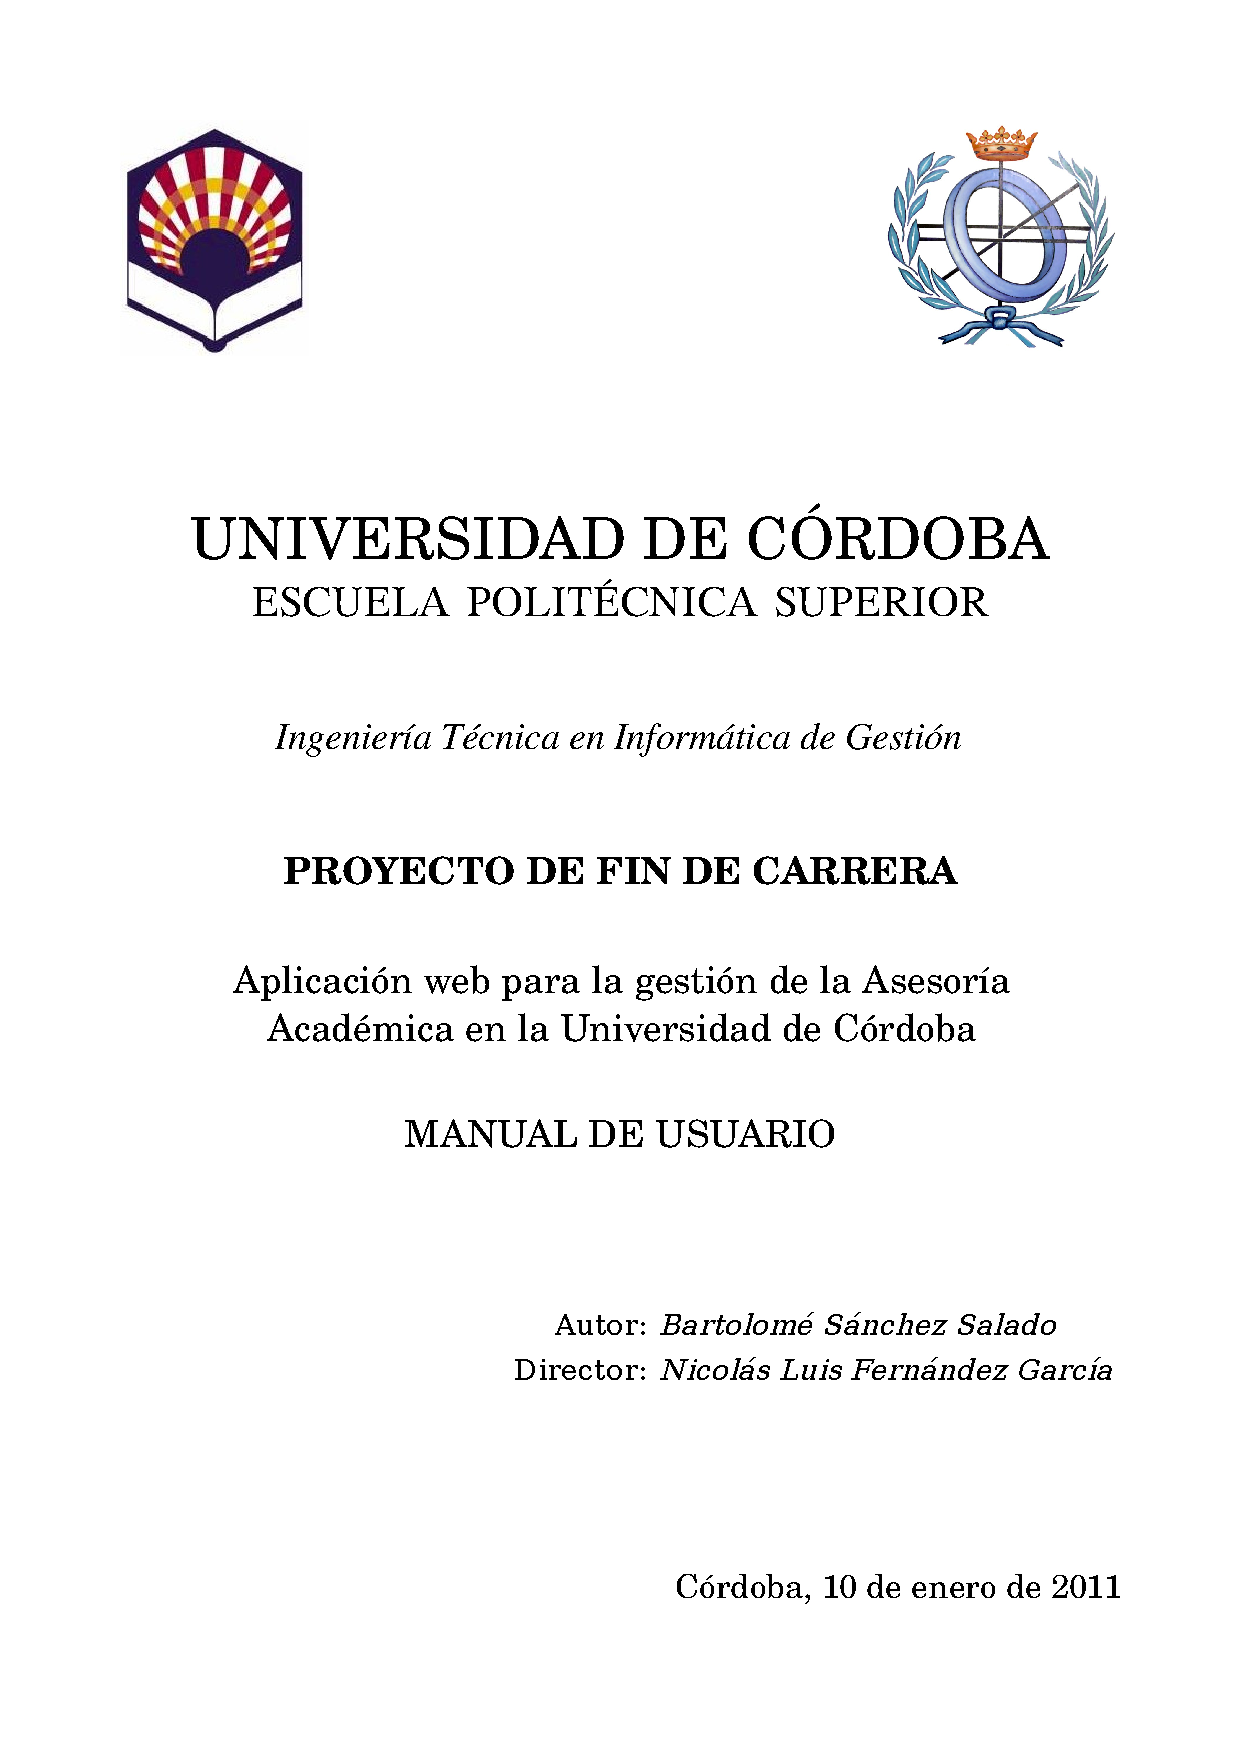
\includepdf[]{Portada/portada_manual_usuario.pdf}
   \cleardoublepage
   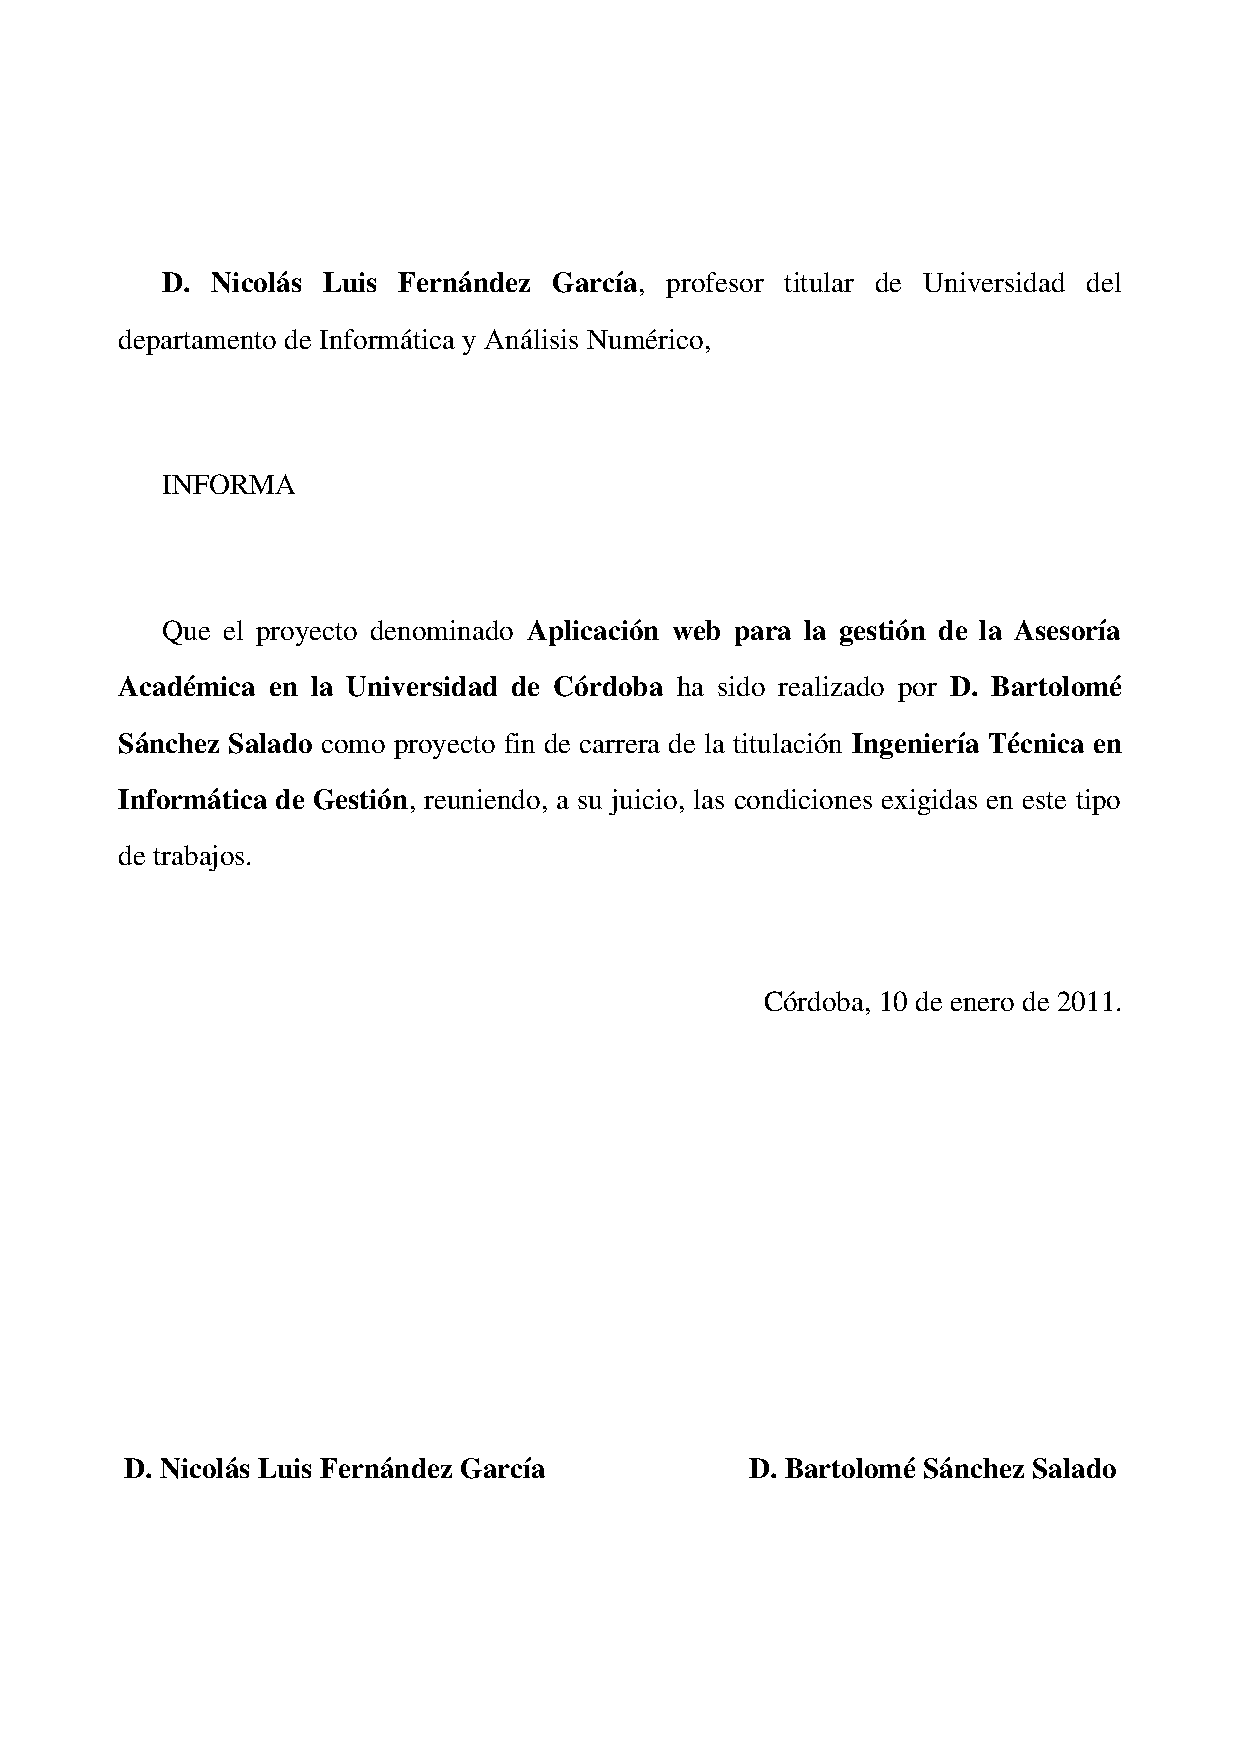
\includepdf[]{Portada/informe_director.pdf}

   \setcounter{page}{0}
   \cleardoublepage

   \pagenumbering{roman}
   \tableofcontents

   \chapter{Introducción}
   \pagenumbering{arabic}
      \section{Introducción}

  \paragraph{}En este capítulo se muestra una visión detallada del
  comportamiento del sistema de manera que sea entendible tanto por el usuario
  final como por los desarrolladores, mediante una representación de cómo fluye
  la información por el sistema desde su entrada hasta su salida.

  \paragraph{}Para realizar esta representación, se utilizarán una serie de
  Diagramas de Flujo de Datos (DFD) que son una herramienta que permite
  visualizar un sistema como una red de procesos funcionales, conectados entre
  sí por \textit{conductos} y \textit{tanques de almacenamiento} de datos.
  También se utilizará un Diccionario de Datos que realizará una representación
  de los elementos requeridos o producidos por la aplicación.


   \chapter{Instalación y desinstalación}
      \section{Requisitos del sistema}

  \paragraph{}El equipo donde se vaya a instalar y usar el software debe cumplir
  una serie de requisitos técnicos para un correcto funcionamiento y
  aprovechamiento total de las funciones ofrecidas por el sistema informático.

  \subsection{Requisitos Hardware}

  \paragraph{}Para la instalación de esta aplicación se necesita de un ordenador
  personal con las siguientes características mínimas:

  \begin{itemize}
   \item Procesador Intel 80486 o superior.
   \item 32 MB de memoria RAM.
   \item 50 MB de espacio libre en disco duro.
   \item Lector de CD-ROM.
   \item Teclado y ratón compatibles.
   \item Conexión a internet.
  \end{itemize}


  \subsection{Requisitos Software}

  \paragraph{}Las aplicaciones necesarias para el correcto funcionamiento del
  sistema son las siguientes:

  \begin{itemize}
   \item Debian GNU/Linux 6.0 ``Squeeze'' \cite{debian}.
   \item Python 2.6.6 \cite{python}.
   \item Django 1.2.3 \cite{django}.
   \item PostgreSQL 8.4.5 \cite{postgresql}.
   \item Subversion 1.4.2 \cite{subversion}.
   \item Apache 2.2.16-4 con el módulo \textit{mod\_wsgi} instalado
   \cite{apache}.
  \end{itemize}



      \section{Proceso de instalación}\label{instalacion}

  \paragraph{}Para proceder con la instalación de la aplicación se deben seguir
  los siguientes pasos:

  \begin{enumerate}
   \item Instalación del \textit{framework}.
   \item Instalación del servidor web.
   \item Configuración del servidor web.
   \item Instalación del sistema gestor de bases de datos.
   \item Configuración del sistema gestor de bases de datos.
   \item Configuración del \textit{framework}.
   \item Creación de las tablas necesarias para la base de datos. ¡¡¡FALTA!!!
  \end{enumerate}

  \paragraph{}A continuación pasaremos a explicar en mayor profundidad cada
  uno de los pasos anteriores para guiar al usuario correctamente en el proceso
  de instalación de la aplicación.

  \begin{enumerate}
    \item \textbf{Instalación del \textit{framework}}.
   Para proceder con la instalación del \textit{framework} utilizado,
   \textit{Django}, deberá introducirse en la línea de comandos:

   \begin{verbatim}
   # aptitude install python-django
   \end{verbatim}

   Seguidamente aparecerá el siguiente mensaje:

   \begin{verbatim}
   Se instalarán los siguiente paquetes NUEVOS:
   python-django
   0 paquetes actualizados, 1 nuevos instalados, 0 para eliminar
   y 0 sin actualizar.
   Necesito descargar 0 B/4194 kB de ficheros. Después de
   desempaquetar se usarán 20,3 MB.
   Seleccionando el paquete python-django previamente no
   seleccionado.
   (Leyendo la base de datos ... 199153 files and directories
   currently installed.)
   Desempaquetando python-django
   (de .../python-django_1.2.3-2_all.deb) ...
   Procesando disparadores para man-db ...
   Configurando python-django (1.2.3-2) ...
   Procesando disparadores para python-support ...
   \end{verbatim}

   Si no ha habido ningún error, el \textit{prompt}\footnote{Según Wikipedia
   \cite{wikipedia2}: \textit{``Se llama prompt al carácter o conjunto de
   caracteres que se muestran en una línea de comandos para indicar que está a
   la espera de órdenes. Éste puede variar dependiendo del intérprete de
   comandos y suele ser configurable.''}} volverá a su situación inicial,
   quedando la aplicación correctamente instalada.
    \item \textbf{Instalación del servidor web}.
   Se procede a instalar el servidor web utilizado, \textit{Apache}, junto
   con su módulo \textit{mod\_wsgi}. Este módulo es necesario para que
   \textit{Apache} sea capaz de interpretar el lenguaje \textit{Python}. Para
   llevar a cabo la instalación, escribiremos el siguiente comando:

   \begin{verbatim}
   # aptitude install apache2 libapache2-mod-wsgi
   \end{verbatim}

   Seguidamente aparecerá el siguiente mensaje:

   \begin{verbatim}
   Se instalarán los siguiente paquetes NUEVOS:
   apache2 apache2-mpm-worker{a} apache2-utils{a} apache2.2-bin{a}
   apache2.2-common{a} libapache2-mod-wsgi
   libaprutil1-dbd-sqlite3{a} libaprutil1-ldap{a} ssl-cert{a}
   0 paquetes actualizados, 9 nuevos instalados, 0 para eliminar
   y 0 sin actualizar.
   Necesito descargar 2016 kB de ficheros. Después de
   desempaquetar se usarán 6808 kB.
   ¿Quiere continuar? [Y/n/?]
   \end{verbatim}

   Introduciendo el carácter \textit{Y}, o pulsando \textit{Intro}, se procederá
   con la instalación completa. El sistema devuelve la siguiente información,
   devolviendo el \textit{prompt} a su estado inicial:

   \begin{verbatim}
   Des:1 http://ftp.fr.debian.org/debian/ testing/main
   libaprutil1-dbd-sqlite3 i386 1.3.9+dfsg-5 [27,2 kB]
   Des:2 http://ftp.fr.debian.org/debian/ testing/main
   libaprutil1-ldap i386 1.3.9+dfsg-5 [25,3 kB]
   Des:3 http://ftp.fr.debian.org/debian/ testing/main
   apache2.2-bin i386 2.2.16-4 [1345 kB]
   Des:4 http://ftp.fr.debian.org/debian/ testing/main
   apache2-utils i386 2.2.16-4 [164 kB]
   Des:5 http://ftp.fr.debian.org/debian/ testing/main
   apache2.2-common i386 2.2.16-4 [307 kB]
   Des:6 http://ftp.fr.debian.org/debian/ testing/main
   apache2-mpm-worker i386 2.2.16-4 [2220 B]
   Des:7 http://ftp.fr.debian.org/debian/ testing/main
   apache2 i386 2.2.16-4 [1384 B]
   Des:8 http://ftp.fr.debian.org/debian/ testing/main
   libapache2-mod-wsgi i386 3.3-1 [129 kB]
   Des:9 http://ftp.fr.debian.org/debian/ testing/main
   ssl-cert all 1.0.28 [14,8 kB]
   Descargados 2016 kB en 11s (172 kB/s).
   Preconfigurando paquetes ...
   Seleccionando el paquete libaprutil1-dbd-sqlite3
   previamente no seleccionado.
   (Leyendo la base de datos ... 200625 files and directories
   currently installed.)
   Desempaquetando libaprutil1-dbd-sqlite3
   (de .../libaprutil1-dbd-sqlite3_1.3.9+dfsg-5_i386.deb) ...
   Seleccionando el paquete libaprutil1-ldap previamente no
   seleccionado.
   Desempaquetando libaprutil1-ldap
   (de .../libaprutil1-ldap_1.3.9+dfsg-5_i386.deb) ...
   Seleccionando el paquete apache2.2-bin previamente no
   seleccionado.
   Desempaquetando apache2.2-bin
   (de .../apache2.2-bin_2.2.16-4_i386.deb) ...
   Seleccionando el paquete apache2-utils previamente no
   seleccionado.
   Desempaquetando apache2-utils
   (de .../apache2-utils_2.2.16-4_i386.deb) ...
   Seleccionando el paquete apache2.2-common previamente no
   seleccionado.
   Desempaquetando apache2.2-common
   (de .../apache2.2-common_2.2.16-4_i386.deb) ...
   Seleccionando el paquete apache2-mpm-worker previamente no
   seleccionado.
   Desempaquetando apache2-mpm-worker
   (de .../apache2-mpm-worker_2.2.16-4_i386.deb) ...
   Seleccionando el paquete apache2 previamente no
   seleccionado.
   Desempaquetando apache2
   (de .../apache2_2.2.16-4_i386.deb) ...
   Seleccionando el paquete libapache2-mod-wsgi previamente no
   seleccionado.
   Desempaquetando libapache2-mod-wsgi
   (de .../libapache2-mod-wsgi_3.3-1_i386.deb) ...
   Seleccionando el paquete ssl-cert previamente no
   seleccionado.
   Desempaquetando ssl-cert
   (de .../ssl-cert_1.0.28_all.deb) ...
   Procesando disparadores para man-db ...
   Configurando libaprutil1-dbd-sqlite3 (1.3.9+dfsg-5) ...
   Configurando libaprutil1-ldap (1.3.9+dfsg-5) ...
   Configurando apache2.2-bin (2.2.16-4) ...
   Configurando apache2-utils (2.2.16-4) ...
   Configurando apache2.2-common (2.2.16-4) ...
   Configurando apache2-mpm-worker (2.2.16-4) ...
   Starting web server: apache2.
   Configurando apache2 (2.2.16-4) ...
   Configurando libapache2-mod-wsgi (3.3-1) ...
   Restarting web server: apache2 ... waiting .
   Configurando ssl-cert (1.0.28) ...
   \end{verbatim}

   De esta forma, la aplicación queda correctamente instalada. Además, el
   servidor web se ha iniciado automáticamente. En caso de tener algún problema
   con el inicio del servidor web, se ha de indicar que el comando para
   iniciarlo es:

   \begin{verbatim}
   # /etc/init.d/apache2 start
   \end{verbatim}

   En nuestro caso, como se había iniciado con normalidad, el comando devuelve
   el mensaje:

   \begin{verbatim}
   Starting web server: apache2httpd (pid 13782) already running.
   \end{verbatim}



    \item \textbf{Configuración del servidor web}.
   Para llevar a cabo la configuración del servidor web, debemos hacer uso del
   contenido de la carpeta \textit{/public/} que acompaña al código fuente de
   esta aplicación.

   En primer lugar, para realizar la configuración del servidor \textit{Apache}
   con su módulo \textit{mod\_wsgi} se proporciona al usuario el archivo
   \textit{httpd.conf} situado en \textit{/public/wsgi-script/}. Este archivo
   es necesario sustituirlo por el archivo de configuración de \textit{Apache}
   del mismo nombre, situado en la ruta del sistema \textit{/etc/apache2/}. Para
   realizar dicha sustitución, introducimos el siguiente comando:

   \begin{verbatim}
   # cp /ruta-proyecto/public/wsgi-scripts/httpd.conf /etc/apache2/
   \end{verbatim}

   Nótese que \textit{ruta-proyecto} debe ser la ruta absoluta al directorio
   \textit{/proyecto/} que contiene el código fuente proporcionado por esta
   aplicación.

   Este archivo hay que modificarlo para configurar correctamente el servidor
   web, ya que hay que tener en cuenta la ruta absoluta del código fuente de
   la aplicación. Para ello, editamos el fichero con nuestro editor favorito
   (en este caso Nano \cite{nano}), teniendo en cuenta de que necesitamos
   permisos de administrador del sistema:

   \begin{verbatim}
   # nano /etc/apache2/httpd.conf
   \end{verbatim}

   Una vez dentro, debemos sustituir la cadena \textit{/ruta-proyecto/} por
   la ruta absoluta donde tengamos almacenado nuestro código fuente. Es decir,
   un nivel superior de donde se encuentra el directorio \textit{/proyecto/}
   proporcionado por el código fuente de esta aplicación.

   Además, es necesario establecer el archivo de configuración para el módulo
   \textit{mod\_wsgi} accesible para \textit{Apache}. Por lo que realizaremos
   una copia al directorio empleado para tal fin:

   \begin{verbatim}
   # cp -R /ruta-proyecto/public/wsgi-script/ /var/www/
   \end{verbatim}

   El archivo que contiene esta carpeta también es necesario modificarlo, por
   lo que escribimos:

   \begin{verbatim}
   # nano /var/www/wsgi-scripts/django.wsgi
   \end{verbatim}

   Y una vez dentro del editor sustituimos \textit{/ruta-proyecto/} (nótese que
   aparece dos veces en el fichero) por la ruta absoluta donde tengamos
   almacenado nuestro código fuente. Es decir, un nivel superior de donde se
   encuentra el directorio \textit{/proyecto/} proporcionado por el código
   fuente de esta aplicación.

   Llegados a este punto es necesario proporcionar a \textit{Apache} los
   archivos multimedia (imágenes y hojas de estilo) necesarias para la ejecución
   de la aplicación. Para realizar dicha acción, introduciremos por línea de
   comandos:

   \begin{verbatim}
   # cp -R /ruta-proyecto/public/media /var/www/
   \end{verbatim}

   Reiniciaremos \textit{Apache} para comprobar que los cambios han tenido
   efecto:

   \begin{verbatim}
   # /etc/init.d/apache2 restart
   \end{verbatim}

   Lo que provocará el siguiente mensaje, si no hay errores:

   \begin{verbatim}
   Restarting web server: apache2 ... waiting .
   \end{verbatim}

   Para comprobar que todo ha ido bien, abriremos un navegador e introduciremos
   la URL \textit{http://localhost/asesorias/}. Si se ha realizado la
   instalación satisfactoriamente, debería aparecer la pantalla principal
   de la aplicación vista en el capítulo \ref{pantallaPrincipal},
   \textit{Página principal}.
    \item \textbf{Instalación del sistema gestor de bases de datos}.
   Se procede a instalar el sistema gestor de bases de datos utilizado,
   \textit{PostgreSQL}. Para llevar a cabo la instalación, escribiremos el
   siguiente comando:

   \begin{verbatim}
   # aptitude install postgresql
   \end{verbatim}

   Seguidamente aparecerá el siguiente mensaje:

   \begin{verbatim}
   Se instalarán los siguiente paquetes NUEVOS:
   postgresql postgresql-8.4{a} postgresql-common{a}
   0 paquetes actualizados, 3 nuevos instalados, 0 para eliminar
   y 0 sin actualizar.
   Necesito descargar 5344 kB de ficheros. Después de
   desempaquetar se usarán 15,7 MB.
   ¿Quiere continuar? [Y/n/?]
   \end{verbatim}

   Introduciendo el carácter \textit{Y}, o pulsando \textit{Intro}, se procederá
   con la instalación completa. El sistema devuelve la siguiente información,
   devolviendo el \textit{prompt} a su estado inicial:

   \begin{verbatim}
   Des:1 http://ftp.fr.debian.org/debian/ testing/main
   postgresql-common all 113 [127 kB]
   Des:2 http://ftp.fr.debian.org/debian/ testing/main
   postgresql-8.4 i386 8.4.5-0squeeze2 [5198 kB]
   Des:3 http://ftp.fr.debian.org/debian/ testing/main
   postgresql all 8.4.5-0squeeze2 [18,2 kB]
   Descargados 5344 kB en 10s (526 kB/s).
   Preconfigurando paquetes ...
   Seleccionando el paquete postgresql-common previamente
   no seleccionado.
   (Leyendo la base de datos ... 201096 files and directories
   currently installed.)
   Desempaquetando postgresql-common
   (de .../postgresql-common_113_all.deb) ...
   Seleccionando el paquete postgresql-8.4 previamente
   no seleccionado.
   Desempaquetando postgresql-8.4
   (de .../postgresql-8.4_8.4.5-0squeeze2_i386.deb) ...
   Seleccionando el paquete postgresql previamente
   no seleccionado.
   Desempaquetando postgresql
   (de .../postgresql_8.4.5-0squeeze2_all.deb) ...
   Procesando disparadores para man-db ...
   Configurando postgresql-common (113) ...
   Starting PostgreSQL 8.4 database server: main.
   Configurando postgresql-8.4 (8.4.5-0squeeze2) ...
   update-alternatives: using
   /usr/share/postgresql/8.4/man/man1/postmaster.1.gz to
   provide /usr/share/man/man1/postmaster.1.gz
   (postmaster.1.gz) in auto mode.
   Starting PostgreSQL 8.4 database server: main.
   Configurando postgresql (8.4.5-0squeeze2) ...
   \end{verbatim}

   De esta forma, la aplicación queda correctamente instalada.

    \item \textbf{Configuración del sistema gestor de bases de datos}.
   Se procede a configurar el sistema gestor de bases de datos utilizado,
   \textit{PostgreSQL}.Para llevar a cabo la configuración, debemos editar
   el archivo \textit{pg\_hba.conf} situado en
   \textit{/etc/postgresql/8.4/main/}. Por lo tanto:

   \begin{verbatim}
   # nano /etc/postgresql/8.4/main/pg_hba.conf
   \end{verbatim}

   Una vez dentro, debemos añadir al final del fichero la siguiente línea:

   \begin{verbatim}
   host  asesorias   [usuario]   127.0.0.1/32   [método]
   \end{verbatim}

   Nótese que hay que sustituir \textit{[usuario]} por el nombre de usuario del
   sistema que queremos que administre nuestra aplicación. También será
   necesario sustituir \textit{[método]} por el tipo de método de cifrado de la
   contraseña del usuario de PostgreSQL (normalmente md5). Si tiene problemas
   creando usuarios en PostgreSQL con permisos para leer y escribir bases de
   datos, por favor, diríjase a la documentación oficial de PostgreSQL
   \cite{postgresql}.
    \item \textbf{Configuración del \textit{framework}}.
   Llegados a este punto es necesario configurar el \textit{framework}
   utilizado, \textit{Django}, para que le sea posible conectarse a la base de
   datos que acabamos de configurar. Para ello, debemos editar el archivo
   \textit{settings.py} que se encuentra en la carpeta \textit{proyecto} del
   código fuente que proporciona esta aplicación. Para ello:

   \begin{verbatim}
   $ nano /ruta-proyecto/proyecto/settings.py
   \end{verbatim}

   Una vez dentro, debemos localizar las líneas:

   \begin{verbatim}
   DATABASE_USER = ''
   DATABASE_PASSWORD = ''
   \end{verbatim}

   Se debe introducir el nombre de usuario PostgreSQL válido y la contraseña
   que utilizamos para tener acceso de lectura y escritura para nuestra base
   de datos \textit{asesorías}. Con esto estaría completa la configuración
   del \textit{framework Django}.

%     Creación tablas.
  \end{enumerate}

  \paragraph{}Una vez completados todos los pasos anteriores, la aplicación
  quedaría instalada completamente y funcionando.
      \section{Proceso de desinstalación}


   \chapter{Características de la interfaz}
      \section{Introducción}

  \paragraph{}En este capítulo se muestra una visión detallada del
  comportamiento del sistema de manera que sea entendible tanto por el usuario
  final como por los desarrolladores, mediante una representación de cómo fluye
  la información por el sistema desde su entrada hasta su salida.

  \paragraph{}Para realizar esta representación, se utilizarán una serie de
  Diagramas de Flujo de Datos (DFD) que son una herramienta que permite
  visualizar un sistema como una red de procesos funcionales, conectados entre
  sí por \textit{conductos} y \textit{tanques de almacenamiento} de datos.
  También se utilizará un Diccionario de Datos que realizará una representación
  de los elementos requeridos o producidos por la aplicación.

      \section{Página principal}\label{paginaPrincipal}

  \paragraph{}Desde esta página se podrá acceder a cada una de las zonas de las
  que se compone la aplicación (Administrador principal, Administrador de
  centro, Asesor y Alumno). Además se podrá acceder a la opción de recordar la
  contraseña de un usuario. La página principal de la aplicación puede
  observarse en la figura \ref{capturaPaginaPrincipal}.

  \begin{figure}[!ht]
    \begin{center}
      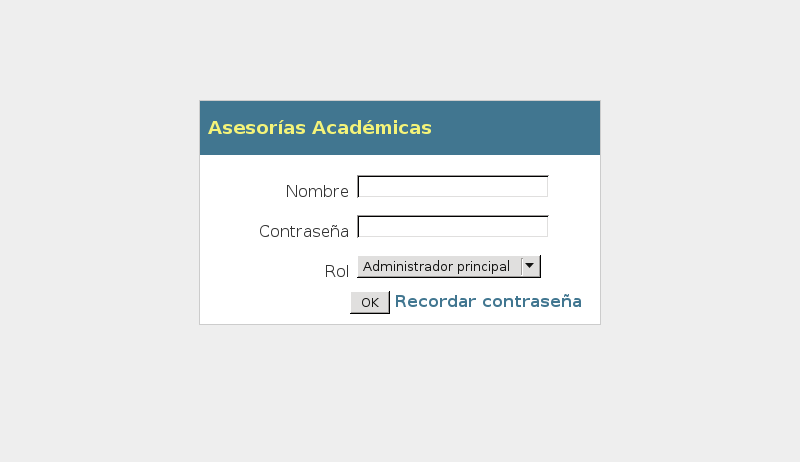
\includegraphics[scale=0.55]{3.Caracteristicas_Interfaz/3.2.Pagina_Principal/pagina_principal.png}
      \caption{Captura de pantalla de la página principal.}
      \label{capturaPaginaPrincipal}
    \end{center}
  \end{figure}

      \section{Gestión de la información}

  \paragraph{}Para todas y cada una de las zonas de las que se compone esta
  aplicación (Administrador principal, Administrador de centro, Asesor y
  Alumno), la interfaz compartirá bastantes detalles en común, diferenciándose
  cada una de ellas del resto en el contenido que puede ver y gestionar el
  usuario que está ejecutando la aplicación, teniendo en cuenta el rol con el
  que participa. Por ejemplo, un usuario asesor no podrá ver determinadas zonas
  para la creación de una nueva titulación, ya que es una tarea que no le
  concierne.

  \paragraph{}Teniendo en cuenta lo anterior, a continuación se muestra una
  captura de pantalla para ejemplificar el diseño de la interfaz común a todas
  las zonas de la aplicación. Se ha utilizado la zona del Administrador
  principal por ser la más completa; pero, como se ha comentado antes, el resto
  de zonas comparten los mismos criterios de diseño, por lo cual la
  navegabilidad y usabilidad no varía entre zonas. La figura
  \ref{capturaGestionInformacion} muestra un ejemplo del diseño de la interfaz
  común.

  \begin{figure}[!ht]
    \begin{center}
      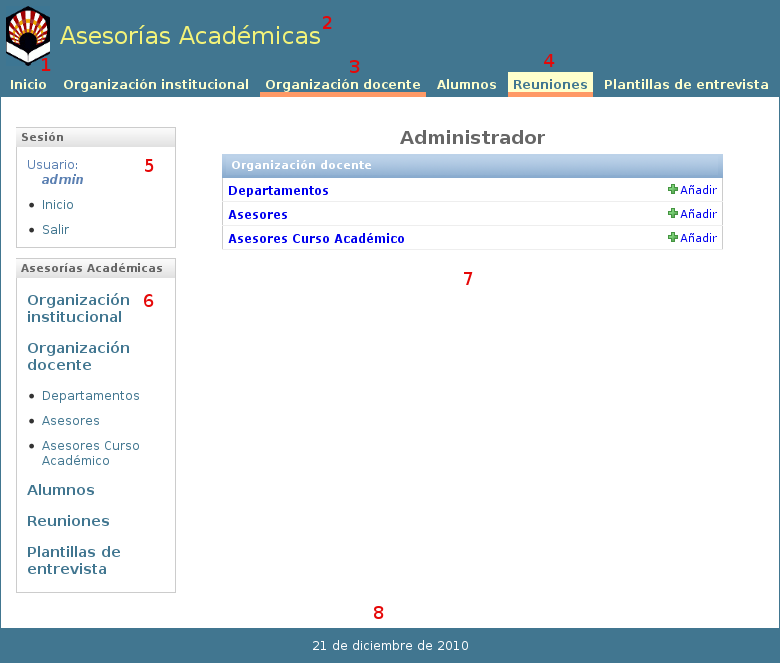
\includegraphics[scale=0.6]{12.Disenyo_Interfaz/12.3.Gestion_Informacion/gestion_informacion.png}
      \caption{Captura de pantalla de la gestión de la información.}
      \label{capturaGestionInformacion}
    \end{center}
  \end{figure}


  \paragraph{}Los elementos de la interfaz a destacar están señalados en la
  imagen con números. A continuación se pasan a detallar:

  \begin{enumerate}
    \item \textbf{Logotipo de la Universidad de Córdoba}. Se trata de un
    enlace que, al pinchar sobre él, nos lleva directamente a la página
    principal de la Universidad de Córdoba (\url{http://www.uco.es}).
    \item \textbf{Nombre completo de la aplicación}.
    \item \textbf{Sección activa}. Se trata de la sección de la aplicación donde
    se encuentra el usuario en un momento determinado.
    \item \textbf{Ir a sección}. Se activa cuando el cursor del ratón se
    encuentra encima del enlace a una determinada sección. Si pulsamos el botón
    del ratón, navegaremos hasta la sección indicada.
    \item \textbf{Menú de sesión}. Este menú contiene detalles acerca de la
    sesión que se encuentra ejecutando en un momento determinado.
    \begin{itemize}
      \item Para todas las zonas de la aplicación (Administrador principal,
      Administrador de centro, Asesor y Alumno), estará visible el nombre de
      usuario que ha iniciado la sesión, así como un enlace directo para ir al
      inicio de cada zona, y un enlace para salir de la sesión, el cual
      desconecta al usuario del sistema.
      \item Para la zona del administrador de centro, se mostrará, además,
      el centro que sea objeto de administración en ese momento.
      \item Para las zonas de Asesor y Alumno, se mostrará, además, el curso
      académico que sea objeto de administración en ese momento.
    \end{itemize}

    \item \textbf{Menú de secciones}. Es un menú de accesos rápidos para las
    distintas opciones de las que se compone la sección en la que se encuentra
    el usuario en un determinado momento, así como accesos al resto de
    secciones de la aplicación.
    \item \textbf{Contenido}. En la zona de contenido se mostrará la distinta
    información que sea necesario detallar en cada momento, teniendo en cuenta
    dónde se encuentre el usuario en un determinado momento.
    \item \textbf{Pie de página}. Zona utilizada para exponer alguna otra
    información que se quiera reflejar. Para esta aplicación se ha utilizado
    la fecha actual como información en el pie de página.
  \end{enumerate}

  \subsection{Lista de elementos}

  \paragraph{}La figura \ref{capturaListaElementos} muestra un ejemplo de
  listado de elementos. Como se puede observar, además aparecen elementos
  importantes que es necesario comentar:

  \begin{itemize}
   \item \textbf{Crear nuevos elementos}. Si el usuario dispone de los permisos
   necesarios aparecerá un icono, representado por una cruz verde junto con el
   texto \textit{Añadir nuevo}, que permitirá la adición de nuevos elementos.
   \item \textbf{Generar PDF}. Exporta el listado actual al formato PDF.
   \item \textbf{Búsqueda}. Se permite realizar búsquedas entre los elementos
   que componen la lista mostrada. La figura \ref{capturaBusquedaElementos}
   muestra un ejemplo de búsqueda de elementos.
   \begin{figure}[!ht]
    \begin{center}
      \fbox{
        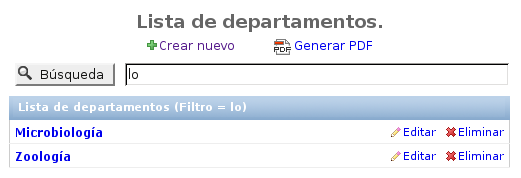
\includegraphics[scale=0.6]{12.Disenyo_Interfaz/12.3.Gestion_Informacion/12.3.1.Lista_Elementos/busqueda_elementos.png}
      }
      \caption{Captura de pantalla de una búsqueda de elementos.}
      \label{capturaBusquedaElementos}
    \end{center}
  \end{figure}
   \item \textbf{Ordenamiento}. Como cabecera de la lista de elementos,
   aparecerá el nombre del conjunto de elementos junto con una flecha indicando
   el tipo de ordenamiento: ascendente o descendente. Si se trata de elementos
   de tipo cadena su ordenamiento se realizará por orden alfabético, y si se
   trata de elementos numéricos de mayor a menor y viceversa.
   \item \textbf{Editar elemento}. Si el usuario dispone de los permisos
   necesarios aparecerá un icono, representado por un lápiz junto con el texto
   \textit{Editar}, que permitirá editar el elemento indicado.
   \item \textbf{Eliminar elemento}. Si el usuario dispone de los permisos
   necesarios aparecerá un icono, representado por una cruz roja girada 45
   grados con respecto a la vertical junto con el texto \textit{Eliminar}, que
   permitirá eliminar el elemento indicado, previa confirmación.
  \end{itemize}

  \begin{figure}[!ht]
    \begin{center}
      \fbox{
        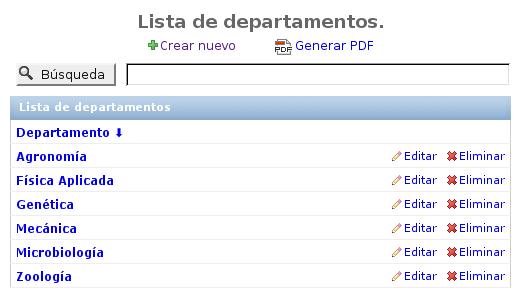
\includegraphics[scale=0.6]{12.Disenyo_Interfaz/12.3.Gestion_Informacion/12.3.1.Lista_Elementos/lista_elementos.png}
      }
      \caption{Captura de pantalla de un listado de elementos.}
      \label{capturaListaElementos}
    \end{center}
  \end{figure}
  \subsection{Adición de elementos}

  \paragraph{}La figura \ref{capturaAdicionElementos} muestra un ejemplo de
  creación de un nuevo elemento. Se puede observar que los campos que dependen
  de otras entidades vienen representados por una lista desplegable, donde se
  debe elegir el elemento al que hacer referencia. El resto de campos se
  introducirán a través de cajas de texto. Por último aparece un botón
  denominado \textit{Confirmar}, el cual intentará crear el elemento en el
  sistema.

  \begin{figure}[!ht]
    \begin{center}
      \fbox{
        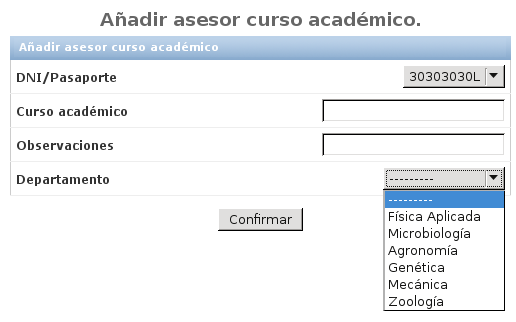
\includegraphics[scale=0.6]{3.Caracteristicas_Interfaz/3.3.Gestion_Informacion/3.3.2.Adicion_Elementos/adicion_elementos.png}
      }
      \caption{Captura de pantalla de la creación de un nuevo elemento.}
      \label{capturaAdicionElementos}
    \end{center}
  \end{figure}

  \item Prueba de actualización de elementos.
  \begin{itemize}
    \item \textbf{Descripción:} Comprobación de actualización de elementos
    en el sistema por los usuarios autorizados. Se ha comprobado la
    actualización de los siguientes elementos para los usuarios indicados a
    continuación:

    \begin{itemize}
      \item Administrador principal.
      \begin{itemize}
        \item Centro.
        \item Administrador de centro.
        \item Centro - Administrador de centro.
        \item Titulación.
        \item Asignatura.
        \item Asignatura Curso Académico.
        \item Departamento.
        \item Asesor.
        \item Asesor Curso Académico.
        \item Alumno.
        \item Alumno Curso Académico.
        \item Matrícula.
        \item Calificación Convocatoria.
        \item Reunión.
        \item Reunión - Pregunta de asesor.
        \item Reunión - Pregunta oficial.
        \item Plantilla de entrevista oficial.
        \item Pregunta oficial.
        \item Plantilla de entrevista de asesor.
        \item Pregunta de asesor.
      \end{itemize}
      \item Administrador de centro.
      \begin{itemize}
        \item Contraseña.
        \item Titulación.
        \item Asignatura.
        \item Matrícula.
        \item Calificación Convocatoria.
      \end{itemize}
      \item Asesor.
      \begin{itemize}
        \item Plantilla de asesor.
        \item Pregunta de asesor.
        \item Reunión individual.
        \item Reunión grupal.
        \item Información personal
        \item Contraseña.
        \item Pregunta de reunión.
      \end{itemize}
      \item Alumno
      \begin{itemize}
        \item Información personal.
        \item Contraseña.
        \item Pregunta de reunión.
      \end{itemize}
    \end{itemize}

    \item \textbf{Problemas encontrados:} No se han encontrado problemas
    funcionales en la actualización de elementos.
    \item \textbf{Soluciones adoptadas:} -
  \end{itemize}



   \chapter{Funcionamiento de la aplicación}

   \chapter{Ejemplos prácticos}

   \listoffigures

   \begin{thebibliography}{xx}

\bibitem{debian} \textbf{Debian GNU/Linux}, 2009.\\
         Sitio web oficial del sistema operativo.\\
         url: \url{http://www.debian.org/}
         [Consulta: 20 junio 2009].
\bibitem{django} \textbf{Django}, 2009.\\
         Sitio oficial del proyecto.\\
         url: \url{http://www.djangoproject.com/}
         [Consulta: 20 junio 2009].
\bibitem{kate} \textbf{Kate}, 2009.\\
         Sitio oficial del editor de textos.\\
         url: \url{http://kate-editor.org/}
         [Consulta: 20 junio 2009].
\bibitem{kile} \textbf{Kile}, 2009.\\
         Sitio oficial del editor de Tex/Latex.\\
         url: \url{http://kile.sourceforge.net/}
         [Consulta: 20 junio 2009].
\bibitem{latex} \textbf{Latex}, 2009.\\
         Sitio oficial del proyecto \LaTeX.\\
         url: \url{http://www.latex-project.org/}
         [Consulta: 20 junio 2009].
\bibitem{microsoft} \textbf{Microsoft}, 2009.\\
         Sitio oficial de la compañía.\\
         url: \url{http://www.microsoft.com/}
         [Consulta: 20 junio 2009].
\bibitem{mysql} \textbf{MySQL}, Sun Microsystems, 2009.\\
         Sitio oficial del sistema gestor de bases de datos.\\
         url: \url{http://www.mysql.com/}
\bibitem{oracle} \textbf{Oracle}, 2009.\\
         Sitio oficial del sistema gestor de bases de datos.\\
         url: \url{http://www.oracle.com/}
         [Consulta: 20 junio 2009].
\bibitem{peterChen} \textbf{Peter Pin-Shan S. Chen}, 1976.\\
         The Entity-Relationship Model: Toward a Unified View of Data. \\
         ACM Transactions on Database Systems. Páginas 9-36.
         ISSN:0362-5915.
\bibitem{php} \textbf{PHP}, 2009.\\
         Sitio oficial del lenguaje.\\
         url: \url{http://www.php.net/}
         [Consulta: 20 junio 2009].
\bibitem{postgresql} \textbf{PostgreSQL}, 2009.\\
         Sitio oficial del sistema gestor de bases de datos.\\
         url: \url{http://www.postgresql.org/}
         [Consulta: 20 junio 2009].
\bibitem{python} \textbf{Python}, 2009.\\
         Sitio oficial del lenguaje.\\
         url: \url{http://www.python.org/}
         [Consulta: 20 junio 2009].
\bibitem{ruby} \textbf{Ruby}, 2009.\\
         Sitio oficial del lenguaje.\\
         url: \url{http://www.ruby-lang.org/}
         [Consulta: 20 junio 2009].
\bibitem{subversion} \textbf{Subversion} , 2009.\\
         Sitio oficial del sistema de control de versiones.\\
         url: \url{http://subversion.tigris.org/}
         [Consulta: 20 junio 2009].
\bibitem{wikipedia} \textbf{Wikipedia}, 2009.\\
         Sitio oficial del proyecto.\\
         url: \url{http://www.wikipedia.org/}
         [Consulta: 20 junio 2009].
 \end{thebibliography}

\end{document}